\chapter{Architectural Views for Suggestions to Improve the Existing System}

\section{Context View}

\subsection{Stakeholders' uses of this view}

There are three main stakeholders of the system: the volunteers, victims, developers. \\

The volunteers use this view to understand how they will help the victims by sharing information with website.
The victims use this view to understand how they can get help to get food, healthcare, etc.
The developers use this view to understand how they can build a bridge between victims and volunteers and how they can achieve to forward the validated information as fast as possible.

\subsection{Context Diagram}

\begin{figure}[H]
    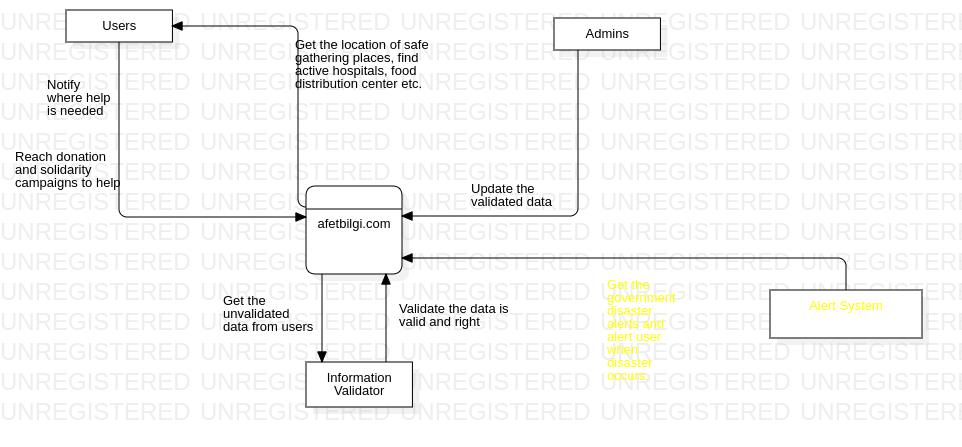
\includegraphics[scale = 0.5]{assets/System Context DiagramSuggestion.png}
    \caption[Suggested System Context Diagram]{Suggested System Context Diagram}
\end{figure}

\subsection{External Interfaces}

\begin{figure}[H]
    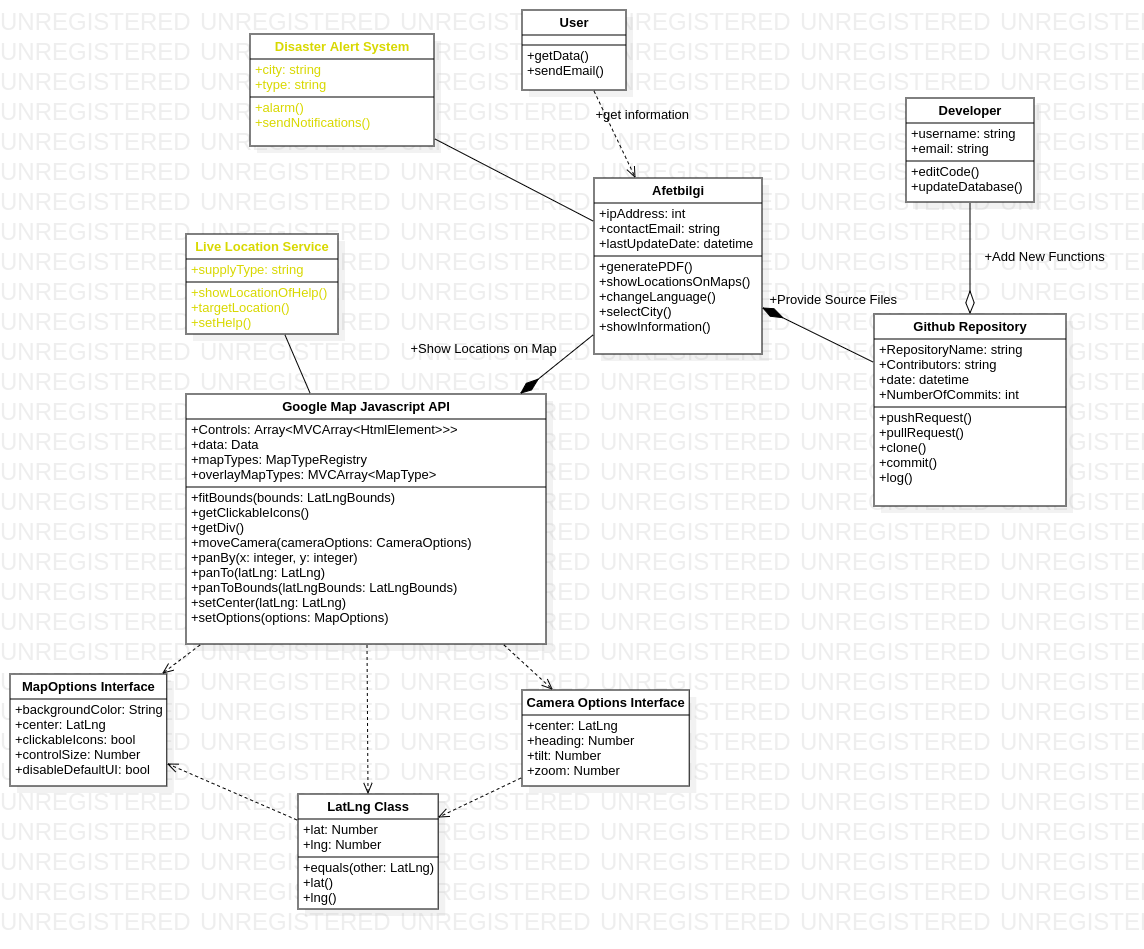
\includegraphics[scale = 0.4]{assets/ExternalInterfaceSuggestion.png}
    \caption[Suggested External Interface]{Suggested External Interface}
\end{figure}

\begin{center}
    \begin{table}[H]
        \begin{tabular}{| m{6cm}| m{8cm} |}
            \hline
            \textbf{Operation} & \textbf{Description} \\
            \hline
            generatePdf & The website generate the pdf which contains the selected city crucial information in compact form as a downloadable file by users.\\
            \hline
            showLocationsOnMaps & Website shows the important locations on the map.\\
            \hline
            changeLanguage & Users can choose a language between Turkish, English, Kurdi and Arabic.\\
            \hline
            selectCity & Website filter the datas according to selected city.\\
            \hline
            showInformations & Shows the information as subparts on the website mainpage.\\
            \hline
            editCode & Developers can edit the code in the source files.\\
            \hline
            updateDatabase & Developers can update the database with the validated information.\\
            \hline
            getData & Users can reach the validated data by using this website.\\
            \hline
            sendEmail & In case of truth of information or error in server, users can send an email.\\
            \hline
            pushRequest & Developers can push the code changes to Github Repository.\\
            \hline
            pullRequest & Developers can pull the code from the Github Repository.\\
            \hline
            clone & Developers can download the code from the Github Repository.\\
            \hline
            commit & Developers can record changes in their code.\\
            \hline
            log & Developers can look at it previous commits.\\
            \hline
            getClickableIcons & Google Maps API gets the icons such as hospital and pharmacies to show on map.\\
            \hline
            \textcolor{yellow}{alarm} & \textcolor{yellow}{Alarm all affected users from disaster.} \\
            \hline
            \textcolor{yellow}{sendNotification} & \textcolor{yellow}{Send notification when the disaster occurs.} \\
            \hline
            \textcolor{yellow}{showLocationsOfHelp} & \textcolor{yellow}{Show locations of coming help on map.} \\
            \hline
            \textcolor{yellow}{targetLocation} & \textcolor{yellow}{Show the aid destination.} \\
            \hline
            \textcolor{yellow}{setHelp} & \textcolor{yellow}{Create an aid to go.} \\
            \hline
        \end{tabular}
        \caption[Suggested External Interface Operation Descriptions]{Suggested External Interface Operation Descriptions}
    \end{table}
\end{center}

\subsection{Interaction scenarios}

\begin{figure}[H]
    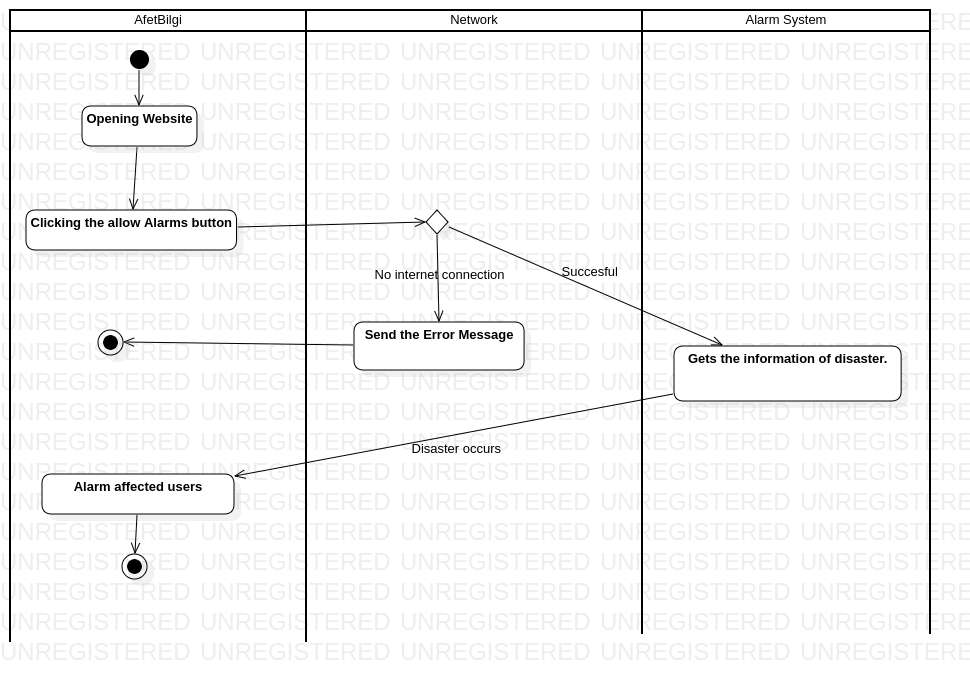
\includegraphics[scale = 0.5]{assets/Activity Diagram Suggestion.png}
    \caption[Suggested Activity Diagram]{Suggested Activity Diagram}
\end{figure}

\section{Functional View}

\subsection{Stakeholders' use of this view}

There are three main stakeholders of the system: the volunteers, victims and developers. \\

The volunteers use this view to find locations which can help to go there or donating money.
The victims especially use this view to make use of Google Maps API since it is very helpful to find all crucial locations in a compact form near them.
The developers use this view to add new functionalities to this system so that they can reach more people and help to faster delivery of aid.

\subsection{Component Diagram}

\begin{figure}[H]
    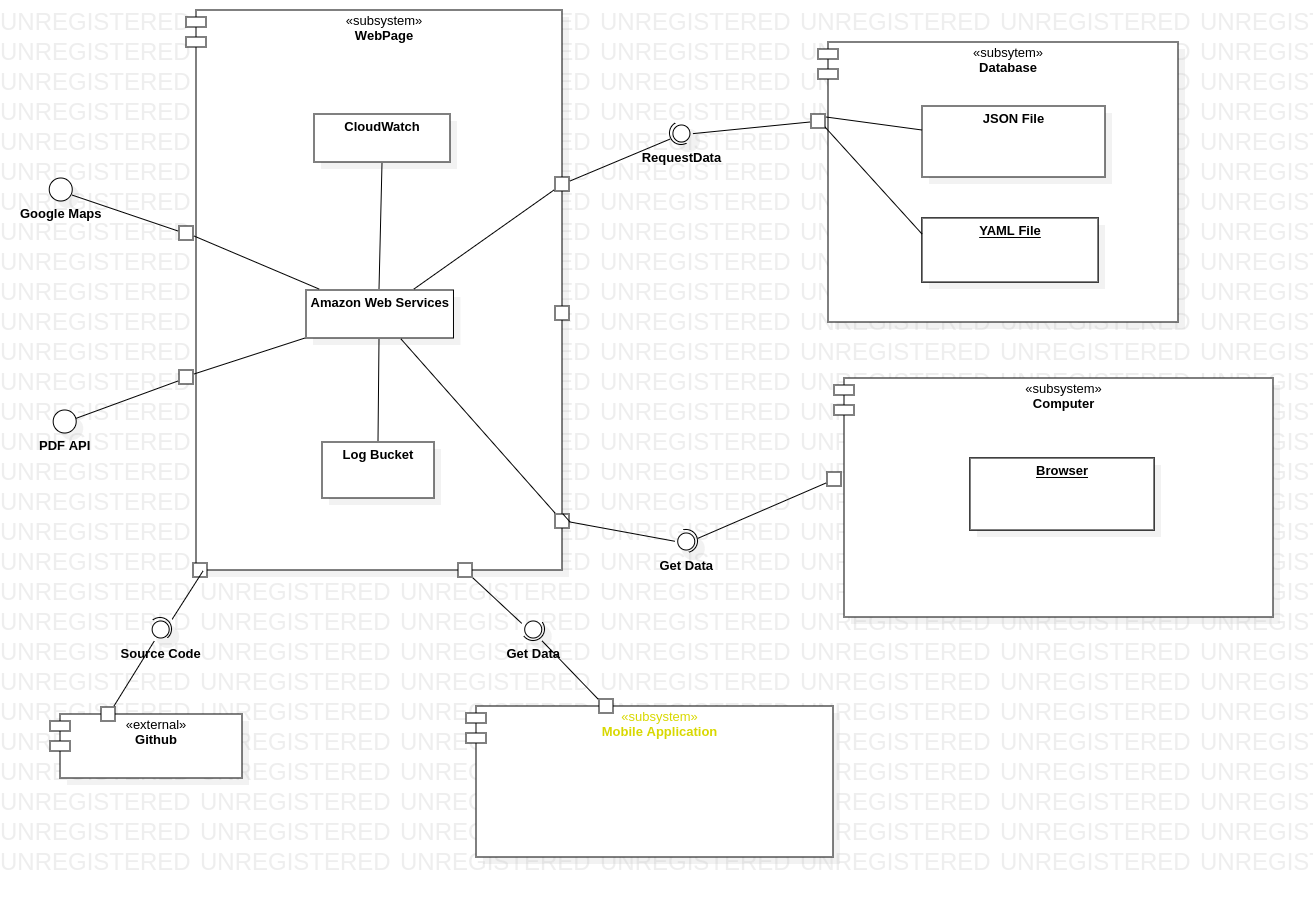
\includegraphics[scale = 0.4]{assets/ComponentDiagramSuggestion.png}
    \caption[Suggested Component Diagram]{Suggested Component Diagram}
\end{figure}

\subsection{Internal Interfaces}

\begin{figure}[H]
    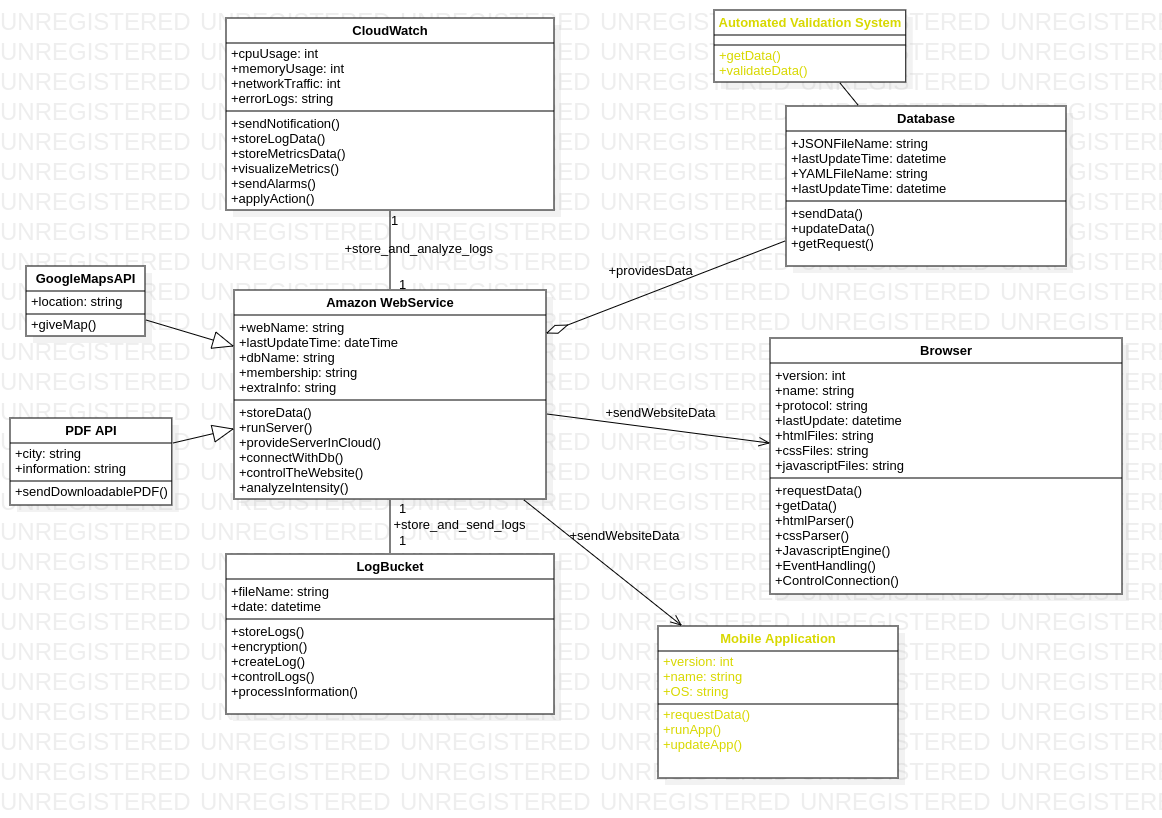
\includegraphics[scale = 0.4]{assets/InternalInterfacesSuggestion.png}
    \caption[Suggested Internal Interfaces]{Suggested Internal Interfaces}
\end{figure}

\begin{center}
    \begin{table}[H]
        \begin{tabular}{| m{6cm}| m{8cm} |}
            \hline
            \textbf{Operation} & \textbf{Description} \\
            \hline
            sendData & Sends a data to a web server.\\
            \hline
            updateData & Update the current database with new data.\\
            \hline
            getRequest & Retrieves a request maded by a server.\\
            \hline
            requestData & Requests data from a server.\\
            \hline
            getData & Retrieves data from a server.\\
            \hline
            htmlParser & Parses and extracts information from HTML documents.\\
            \hline
            cssParser & Parses and extracts information from CSS documents.\\
            \hline
            JavascriptEngine & Executes Javascript code.\\
            \hline
            EventHandling & Handles events triggered by user interactions or system events.\\
            \hline
            ControlConnection & Manages and maintains connections for controlling or communicating with external systems.\\
            \hline
            sendNotification & Sends a notification via email to the user.\\
            \hline
            storeLogData & Stores log data for future analysis.\\
            \hline
            storeMetricsData & Stores metrics or performance data for analysis.\\
            \hline
            visualizeMetrics & Shows metrics or performance data in a visual format.\\
            \hline
            sendAlarms & Sends alarms to notify about specific conditions.\\
            \hline
            storeData & Saves data for future use.\\
            \hline
            runServer & Runs a server.\\
            \hline
            storeLogs & Saves log entries or records for tracking or analysis.\\
            \hline
            encryption & Implements encryption algorithms or techniques to secure data.\\
            \hline
            createLog & Creates log entries or records for system.\\
            \hline
            controlLogs & Manages log entries, including filtering or searching.\\
            \hline
            processInformation & Helps to analyzes information.\\
            \hline
            \textcolor{yellow}{getData} & \textcolor{yellow}{Gets the data for validation.} \\
            \hline
            \textcolor{yellow}{validateData} & \textcolor{yellow}{Validate the data from government or charities system.} \\
            \hline
            \textcolor{yellow}{requestData} & \textcolor{yellow}{Retrieved data for the mobile application.} \\
            \hline
            \textcolor{yellow}{runApp} & \textcolor{yellow}{Run the program in mobile phone.} \\
            \hline
            \textcolor{yellow}{updateApp} & \textcolor{yellow}{Update the program to latest version.} \\
            \hline
        \end{tabular}
        \caption[Internal Interface Operation Descriptions]{Internal Interface Operation Descriptions}
    \end{table}
\end{center}

\subsection{Interaction Patterns}

\begin{figure}[H]
    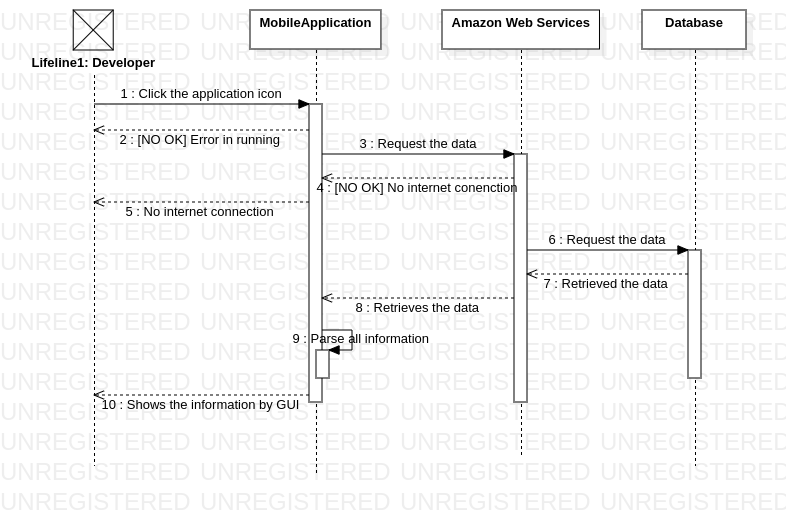
\includegraphics[scale = 0.4]{assets/SequenceDiagramSuggestion.png}    
    \caption[Suggested Sequence Diagram]{Suggested Sequence Diagram}
\end{figure}

\section{Information View}
This view focuses on suggestions to make the website better by adding new functionalities to database.

\subsection{Stakeholders' uses of this view}
\begin{itemize}
    \item Volunteers use this view to understand how an outdated, or wrong data is corrected.
    \item Developers use this view to correct wrong and outdated datas.
\end{itemize}

\subsection{Database Class Diagram}
\begin{figure}[H]
    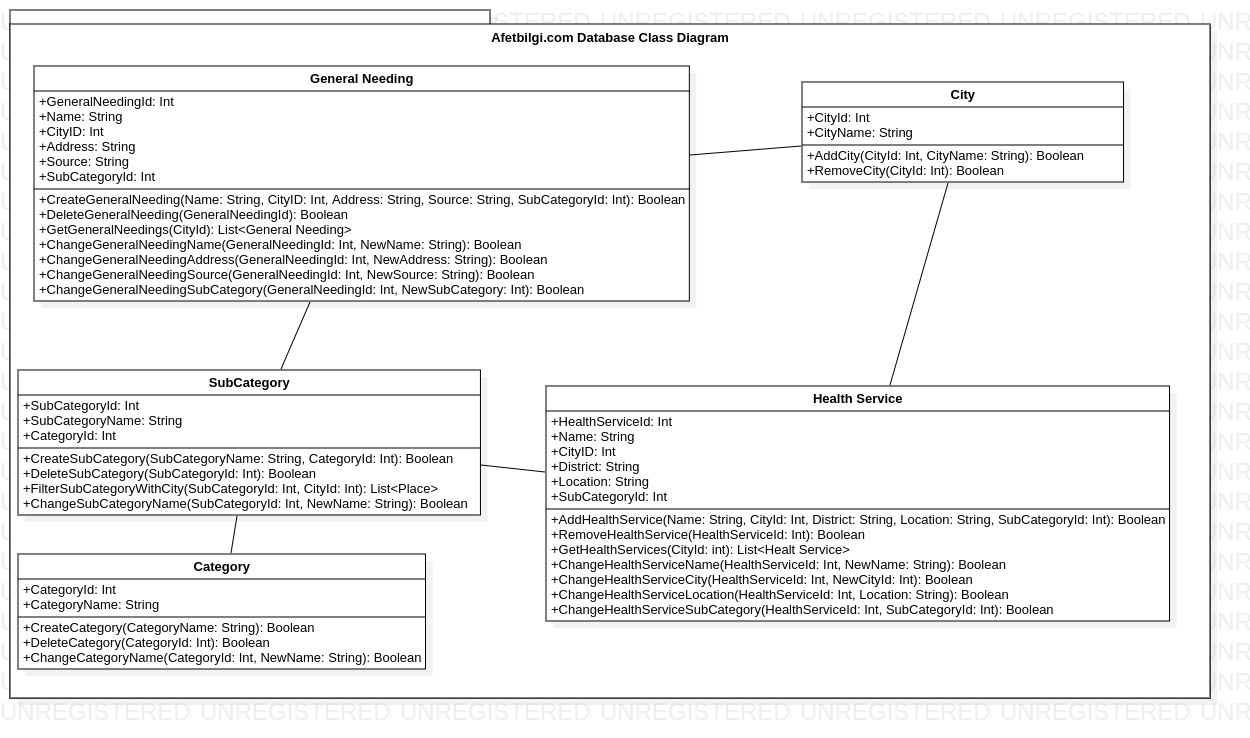
\includegraphics[scale = 0.4]{assets/ClassDiagram2.png}
    \caption[Database Class Diagram With Suggestions]{Database Class Diagram With Suggestions}
\end{figure}

\subsection{Operations on Data}
\begin{table}[H]
    \begin{tabular}{|p{6cm}|p{10cm}|}
        \hline
        \textbf{Operation}   & \textbf{Description}                                                                                                                                    \\
        \hline
        \hline
        ChangeHealthServiceName & Changes name of given healthcare service with given name.\\
        \hline
        ChangeHealthServiceCity & Changes city of given healthcare service.\\
        \hline
        ChangeHealthServiceLocation & Changes location link of given healthcare service. \\
        \hline
        ChangeHealthServiceSubcategory & Changes subcategory of given healthcare service.\\
        \hline
        ChangeSubCategoryname & Change name of subcategory.\\
        \hline
        ChangeGeneralNeedingName & Changes name of general needing.\\
        \hline
        ChangeGeneralNeedingAddress & Changes address link of general needing.\\
        \hline
        ChangeGeneralNeedingSource & Changes source link of general needing.\\
        \hline 
        ChangeGeneralNeedingSubCategory & Changes subcategory of general needing.\\
        \hline
    \end{tabular}
    \caption[Operations on Data with Suggestions]{Operations on Data with Suggestions}
\end{table}


\section{Deployment View}

\subsection{Stakeholders' uses of this view}
\begin{itemize}
    \item Developers can use this view to find out how they can deploy the website when it becomes bigger.
\end{itemize}

\subsection{Deployment Diagram}
\begin{figure}[H]
    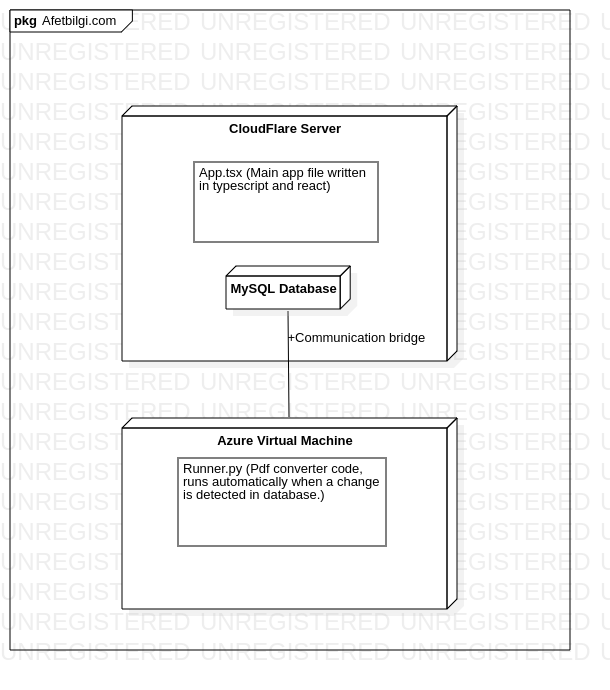
\includegraphics[scale = 0.5]{assets/DeploymentDiagram2.png}
    \caption[Deployment Diagram with Suggestions]{Deployment Diagram with Suggestions}
\end{figure}

\section{Design Rationale}
\begin{itemize}
    \item Live location services can help to improve the link between victims and volunteers.
    \item Mobile application may help to reach more victims and volunteers.
    \item New data operations should be added to fix and correct datas.
    \item Deployment should be seperated on two services, one for deploying the website and handling SQL database, one for updating pdf constantly. So if one of them crashes users can continue to get information by another.
\end{itemize}